\chapter{Main Server configuration}
\label{chapter:server}

In order to control the current features already developed and used in the car it is used a \href{https://www.raspberrypi.org/products/}{Raspberry PI} (currently version 3 model B). The \acrlong{Rpi}, from now on denoted as \acrshort{Rpi}, is a \gls{SBC} affordable and low power, widely used among community and developed by Raspberry Pi Foundation.

\section{Requirements}
For using the \gls{SBC} it is required the following hardware:
\begin{itemize}
	\tightlist
	\item \textbf{Raspberry Pi \gls{SBC}} Recommended version at least 3 since it has a built in wifi.
	\item \textbf{MicroSD card} Recommended with 8Gb capacity at least.
	\item \textbf{Power Supply} Recommended 2.5 Amps . While developing, it is used as the main power for the \gls{SBC}.
	\item \textbf{Host computer (any OS)} with internet and ability to read MicroSD cards.
	\item \textbf{Ethernet cable} for connecting to router/switch for internet access. It can also be used an crossover cable connecting directly to PC if it is able to share internet connection.
\end{itemize}

\section{Initial Preparation}
This preparation will focus on providing instructions to a minimal headless setup. For this reason, the recommended OS image version is the Raspbian Lite.

For this step it is recommended to be used the \href{https://etcher.io/}{Etcher} software for burning the OS image into microSD card. It is assumed the user is familiar with ssh capable software, for example \href{https://www.putty.org/}{Putty}. 
The next steps are mainly based in the documentation guide provided by \cite{raspberry_install_guide}.

\begin{enumerate}
	\tightlist
	\item Download the OS image, Raspbian Lite version in \href{https://www.raspberrypi.org/downloads/raspbian/}{here}
	\item Connect the MicroSD to host computer.
	\item Open Etcher and:
	\begin{enumerate}
		\item Select OS image or zip file that have been downloaded.
		\item Select the SD card you wish to write your image to.
		\item Review your selections and click 'Flash!' to begin writing data to the SD card.
		\item after successful write, continue to next step.
	\end{enumerate}
	\item From microSD card, open the boot partition.
	\item Create a new blank file with name "ssh" without extension. This will allow to enable the ssh daemon at first boot time.
	\item Remove card from host computer and insert on raspberry PI.
	\item Plug in the Ethernet cable and connect the \gls{Rpi} to the same  local network as host computer.
	\item Plug in the power supply to \gls{Rpi}.
\end{enumerate}

If everything went as expected, the \gls{Rpi} will start to boot and prepare the first setup. It will be seen led light blinking indicating activity. After a few minutes, it should be possible to access it remotely via ssh

%-------------------------------------------------------------------------------
% create a remote access setup
%-------------------------------------------------------------------------------

\subsection{Remote access}
The next step is to find the ip address of the \gls{Rpi}. For example, in linux terminal type \colorbox{gray!15}{arp -a}. In figure \ref{arp_example} is seen an output example. In red stroke is shown the \gls{MAC} address of a \gls{Rpi}. Every \gls{MAC} is unique and the first three bytes are fixed in every \gls{Rpi} wich correspond to organizationally unique identifier \cite{mac_wiki} associated to Raspberry Pi Foundation, B8:27:EB \cite{wireshark_mac}.

\begin{figure}[hb]
	\centering
	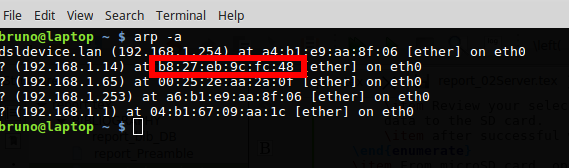
\includegraphics[width=0.7\textwidth]{figures/arp_example}
	\caption{arp -a command example output}
	\label{arp_example}
\end{figure}

Perform the first login with using the default login details as shown in table \ref{tab:default_login}.
Using the discovered ip for the \gls{Rpi}, in Linux, the first login  may be performed using \colorbox{gray!15}{ssh pi@\textless ip-of-Rpi\textgreater} command and entering the default password.
\begin{table}[h]
	\centering
	\begin{tabular}{rl}
		\toprule
		\textbf{username:}& pi\\
		\textbf{password:}& raspberry\\
		\bottomrule
	\end{tabular}
	\caption{Default login details for \gls{Rpi}}
	\label{tab:default_login}
\end{table}

%-------------------------------------------------------------------------------
%  initial update and configurations 
%-------------------------------------------------------------------------------
\subsection{Initial update and configuration}
If the user as been granted with permission to login, the next steps are used to perform a few tweaks.
To do that user must use the command \colorbox{gray!15}{sudo raspi-config}. Example output is seen in figure \ref{fig:raspi_config}.

\begin{itemize}
	\tightlist
	\item Set Keyboard Layout
	\item Update to lastest software
	\item Set Timezone
	\item Set language [optional]
	\item Change default login password
	\item Configure Wifi-zone [if present]
	\item Enable \gls{SPI} for CAN controller
	\item Enable \gls{I2C} for RTC
	\item Set hostname
	\item change default password
	\item change memory for GPU
\end{itemize}

\begin{figure}
	\centering
	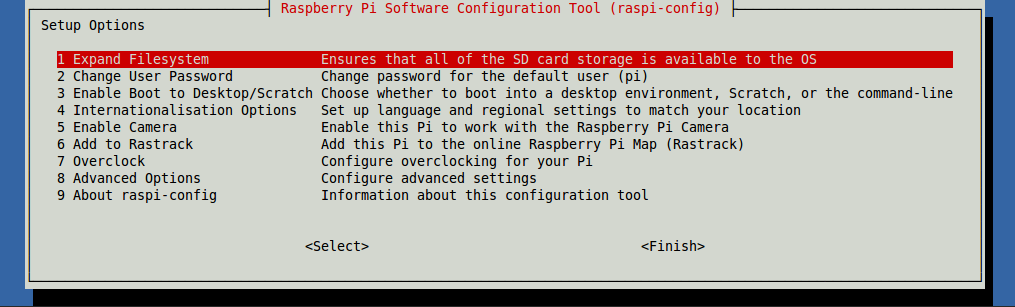
\includegraphics[width=0.7\textwidth]{figures/raspi-config}
	\caption{Raspi-config example output}
	\label{fig:raspi_config}
\end{figure}

The current settings are presented in table \ref{tab:suggested_config}. 

\begin{table}[hb]
	\centering
	\begin{tabular}{rl}
		\toprule
		\textbf{Username:}& pi\\
		\textbf{Password:}& fiatelettra\\
		\textbf{Hostname:}& raspberrypi\\
		\textbf{Language:}& en\_GB.UTF-8 UTF-8\\
	    \textbf{Locale and Timezone:}& Lisbon\\
	    \textbf{Keyboard layout:}& pt\_PT\\
	    \textbf{SPI:}& on\\	
		\textbf{I2C:}& on\\
		\textbf{Memory split:}& 16 (minimum since is running headless)\\
		\bottomrule
	\end{tabular}
	\caption{Suggested details for \gls{Rpi}}
	\label{tab:suggested_config}
\end{table}



%-------------------------------------------------------------------------------
% create a Troubleshooting section
%-------------------------------------------------------------------------------
\section{Troubleshooting}

\begin{description}[style=nextline]
	\item [The command \colorbox{gray!15}{arp -a} do not show my \gls{Rpi}] In that case, try use the \colorbox{gray!15}{sudo nmap -sS 192.168.1.0/24}, assuming the 192.168.1.0/24 is your local network. This is a time consuming command!	
\end{description}

\begin{description}[style=nextline]
	\item [Cannot find my \gls{Rpi} IP. Is it even running?] Maybe there is some problem with boot or bad microSD reading. The easiest solution is to connect a monitor and keyboard. Check messages at boot time. If nothing seems strange, manually login and then check if ehternet connection is ok using \colorbox{gray!15}{ifconfig}
\end{description}


